%----------------------------------------------------------------------------------------
%	PACKAGES AND THEMES
%----------------------------------------------------------------------------------------

\documentclass{beamer}
\mode<presentation> {
	\usetheme{Warsaw}
	\setbeamercolor{page_num_color}{fg=white,bg=blue}

	\defbeamertemplate*{footline}{shadow theme}{%
		\leavevmode%
		\hbox{\begin{beamercolorbox}[wd=.5\paperwidth,ht=2.5ex,dp=1.125ex,leftskip=.3cm plus1fil,rightskip=.3cm]{author in head/foot}%
		    \usebeamerfont{author in head/foot}\hfill\insertshortauthor
		\end{beamercolorbox}%
		\begin{beamercolorbox}[wd=.4\paperwidth,ht=2.5ex,dp=1.125ex,leftskip=.3cm,rightskip=.3cm plus1fil]{title in head/foot}%
		    \usebeamerfont{title in head/foot}\insertshorttitle\hfill%
		\end{beamercolorbox}%
		\begin{beamercolorbox}[wd=.1\paperwidth,ht=2.5ex,dp=1.125ex,leftskip=.3cm,rightskip=.3cm plus1fil]{author in head/foot}%
		\hfill\insertframenumber\,/\,\inserttotalframenumber
		\end{beamercolorbox}}%
		\vskip0pt%
	}
}

\usepackage{amsmath}
\usepackage{amssymb}
\usepackage{graphicx} % Allows including images
\usepackage{booktabs} % Allows the use of \toprule, \midrule and \bottomrule in tables
\usepackage[english]{babel}
\usepackage{graphicx}
\usepackage{listings, lstautogobble}
\usepackage{color}
\usepackage{caption}
\usepackage{verbatim}


%----------------------------------------------------------------------------------------
%	LSTSETTING
%----------------------------------------------------------------------------------------
\lstset{language=C,
    keywordstyle=\color{blue}, 
    morekeywords={then},
    numberstyle=\footnotesize,
    basicstyle=\ttfamily\footnotesize,
    numbers=left,
    stepnumber=1,
    frame=single,
    breaklines=true,
    tabsize=4,
    escapeinside={(*}{*)},
    autogobble=true
}

%----------------------------------------------------------------------------------------
%   TITLE PAGE 
%----------------------------------------------------------------------------------------

\title[Harvesting of Spare Cycles and Storage]
{History-Based Harvesting of Spare Cycles and Storage in Large-Scale Datacenters} % The short title appears at the bottom of every slide, the full title is only on the title page
\author[Yunqi Zhang]
{   Yunqi Zhang, George Prekas, Giovanni Matteo Fumarola,\\
	Marcus Fontoura, Inigo Goiri, Ricardo Bianchini.\\
	{\it University of Michigan and Microsoft Research}
} % Your name
\institute[] % Your institution as it will appear on the bottom of every slide, may be shorthand to save space
{
	12th USENIX symposium on Operating System Design and Implementation \\ % Your institution for the title page
 	\bigskip Presenter: Yi-Ning Chang
}
\date{July 27, 2017} % Date, can be changed to a custom date


\begin{document}

%----------------------------------------------------------------------------------------
%	TITLE PAGE SETTING
%----------------------------------------------------------------------------------------
\begin{frame}[noframenumbering]
    \titlepage % Print the title page as the first slide
\end{frame}

\AtBeginSection[]
  {
  	 \setbeamertemplate{footline}{} 
     \begin{frame}<beamer>[noframenumbering]
     \tableofcontents[currentsection, hideallsubsections]
     \end{frame}
     \setbeamertemplate{footline}{%
		\leavevmode%
		\hbox{\begin{beamercolorbox}[wd=.5\paperwidth,ht=2.5ex,dp=1.125ex,leftskip=.3cm plus1fil,rightskip=.3cm]{author in head/foot}%
		    \usebeamerfont{author in head/foot}\hfill\insertshortauthor
		\end{beamercolorbox}%
		\begin{beamercolorbox}[wd=.4\paperwidth,ht=2.5ex,dp=1.125ex,leftskip=.3cm,rightskip=.3cm plus1fil]{title in head/foot}%
		    \usebeamerfont{title in head/foot}\insertshorttitle\hfill%
		\end{beamercolorbox}%
		\begin{beamercolorbox}[wd=.1\paperwidth,ht=2.5ex,dp=1.125ex,leftskip=.3cm,rightskip=.3cm plus1fil]{author in head/foot}%
		\hfill\insertframenumber\,/\,\inserttotalframenumber
		\end{beamercolorbox}}%
		\vskip0pt%
	}
  }


%------------------------------------------------
% Outline
%------------------------------------------------
\begin{frame}
\frametitle{Outline} % Table of contents slide, comment this block out to remove it
\tableofcontents[hideallsubsections] % Throughout your presentation, if you choose to use \section{} and \subsection{} commands, these will automatically be printed on this slide as an overview of your presentation
\end{frame}


%------------------------------------------------
% Introduction
%------------------------------------------------
\section{Introduction}

% Introduction
\subsection{Introduction}
    \begin{frame}
    \frametitle{Introduction}
		\begin{itemize}
		\item Overprovision resources in datacenters
			\begin{itemize}
			\item Low tail latency requirement
			\item Provisioned for peak load
			\item Unexpected load spikes and failures
			\end{itemize}
		\item A way to increase utilization and reduce costs in datacenters is to co-locate their latency-critical services and batch workloads.
		\item Harvest spare compute cycles and storage space for co-location purpose.
		\end{itemize}
    \end{frame}

% Challenges
\subsection{Challenges}
	\begin{frame}
	\frametitle{Challenges}
		\begin{itemize}
		\item Interactive services ``own'' the servers
		\item Resource availability
			\begin{itemize}
			\item Interactive services performance
			\item Resource availability dynamics - task killing
			\end{itemize}
		\item Data storage co-location
			\begin{itemize}
			\item Data availability
			\item Data durability
			\end{itemize}
		\end{itemize}
	\end{frame}

%------------------------------------------------
% Behavior Patterns
%------------------------------------------------
\section{Behavior Patterns}

% Resource utilization
\subsection{Resource utilization}
	\begin{frame}
	\frametitle{Resource Utilization}
		\begin{itemize}
		\item Identify three main classes of primary tenants.
		\end{itemize}
		\begin{figure}[h!]
		\centering
		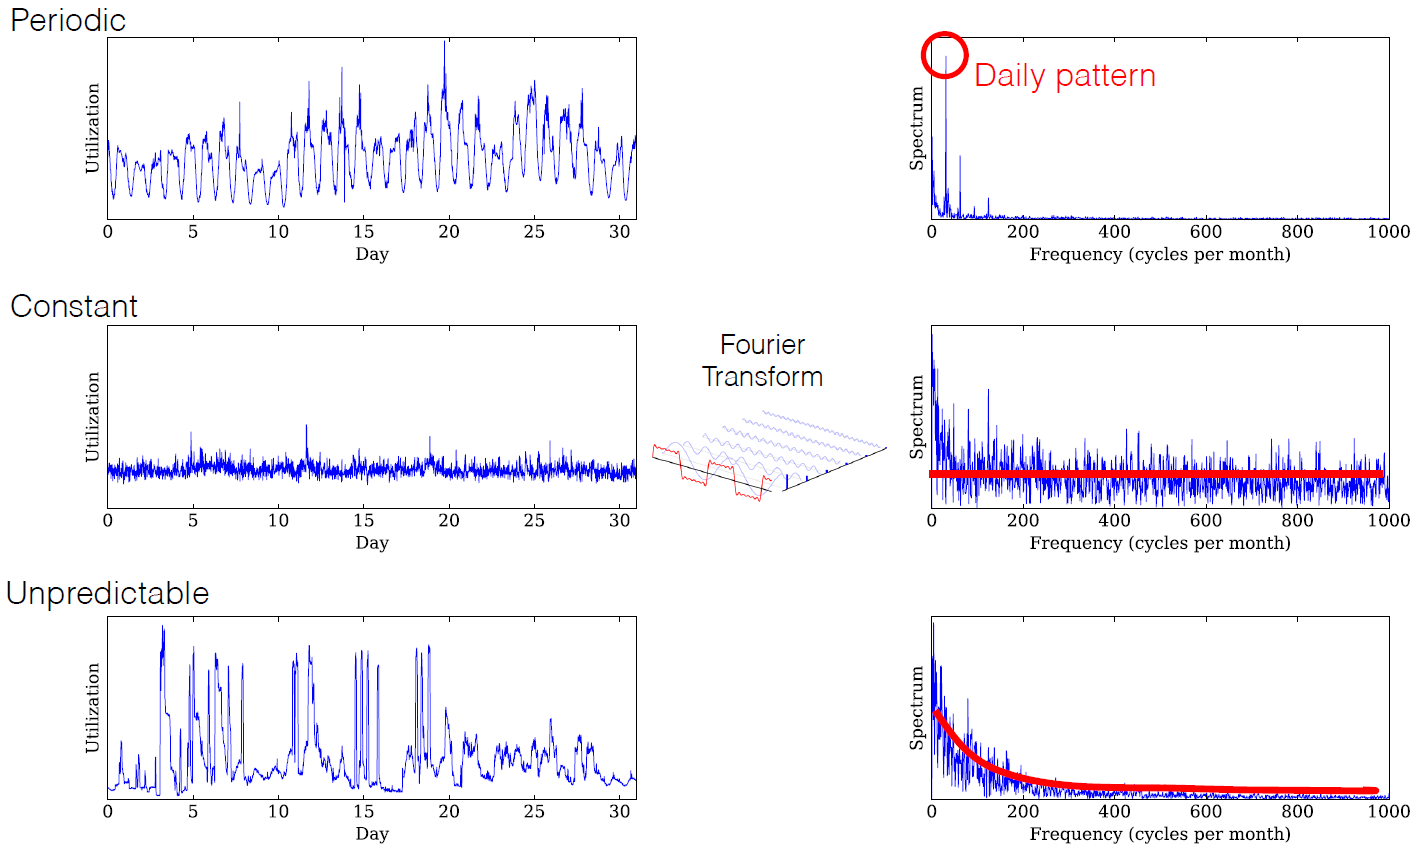
\includegraphics[width=0.8\textwidth]{./figure/pattern.PNG}
		\end{figure}
	\end{frame}

	\begin{frame}
	\frametitle{Resource Utilization}
		\begin{itemize}
		\item Percentages of servers per class.
		\end{itemize}
		\begin{figure}[h!]
		\centering
		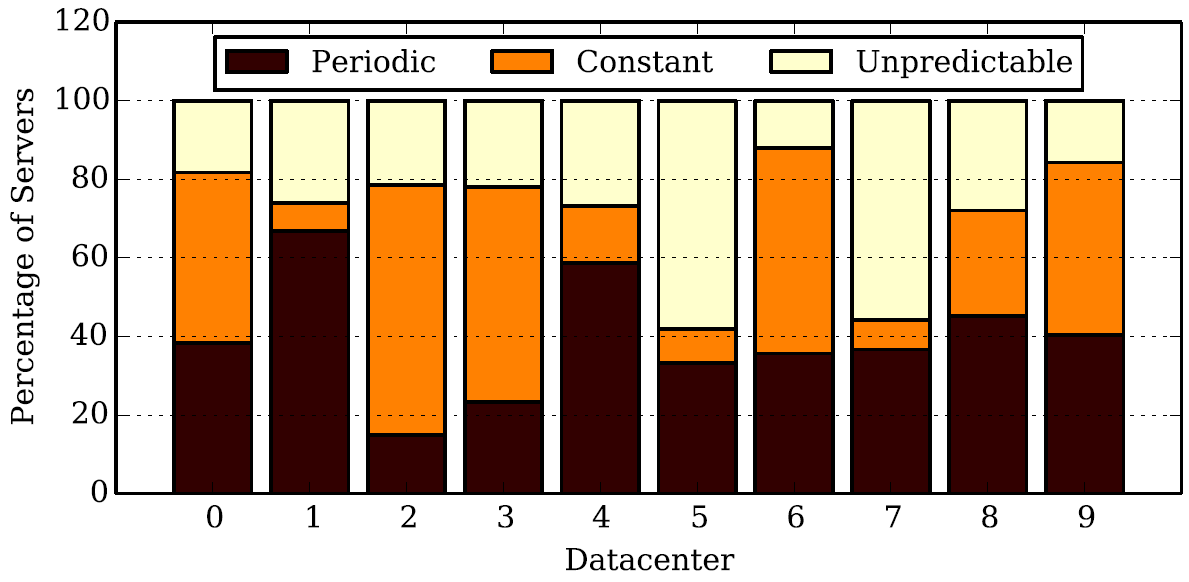
\includegraphics[width=0.8\textwidth]{./figure/datacenter.PNG}
		\end{figure}
	\end{frame}

% Disk reimaging
\subsection{Disk reimaging}
	\begin{frame}
	\frametitle{Disk Reimaging}
		\begin{itemize}
		\item Per-server number of reimages in three years.
		\begin{figure}[h!]
		\centering
		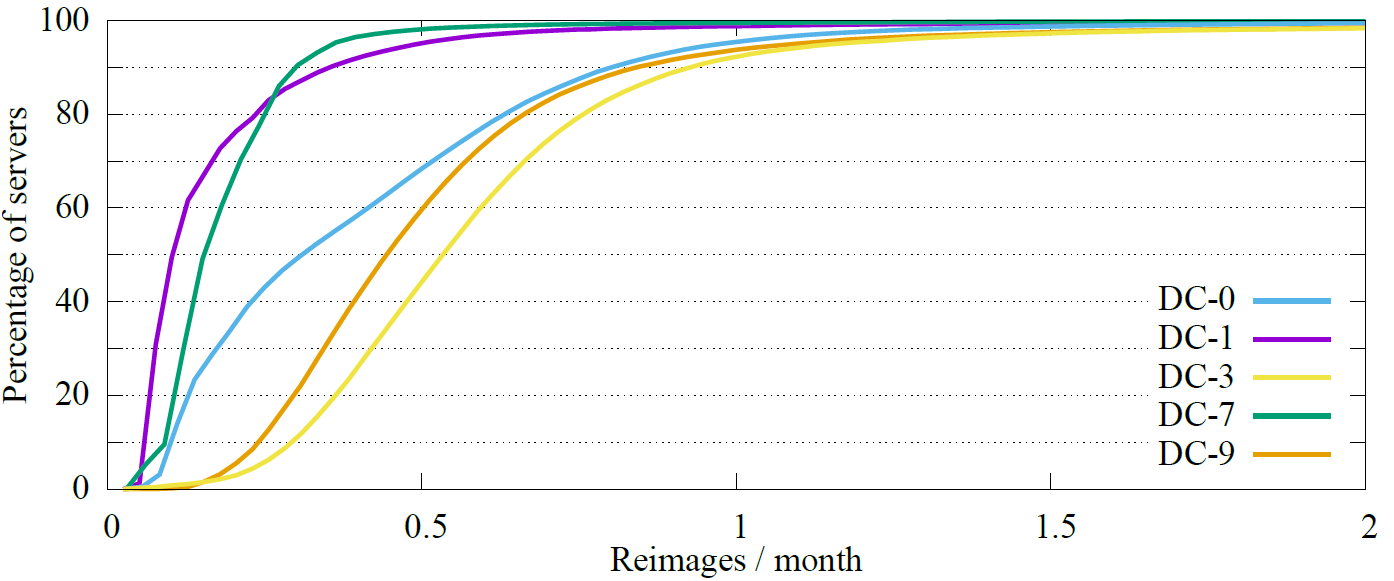
\includegraphics[width=0.5\textwidth]{./figure/reimages1.PNG}
		\end{figure}
		\item Per-tenant number of reimages in three years.
		\begin{figure}[h!]
		\centering
		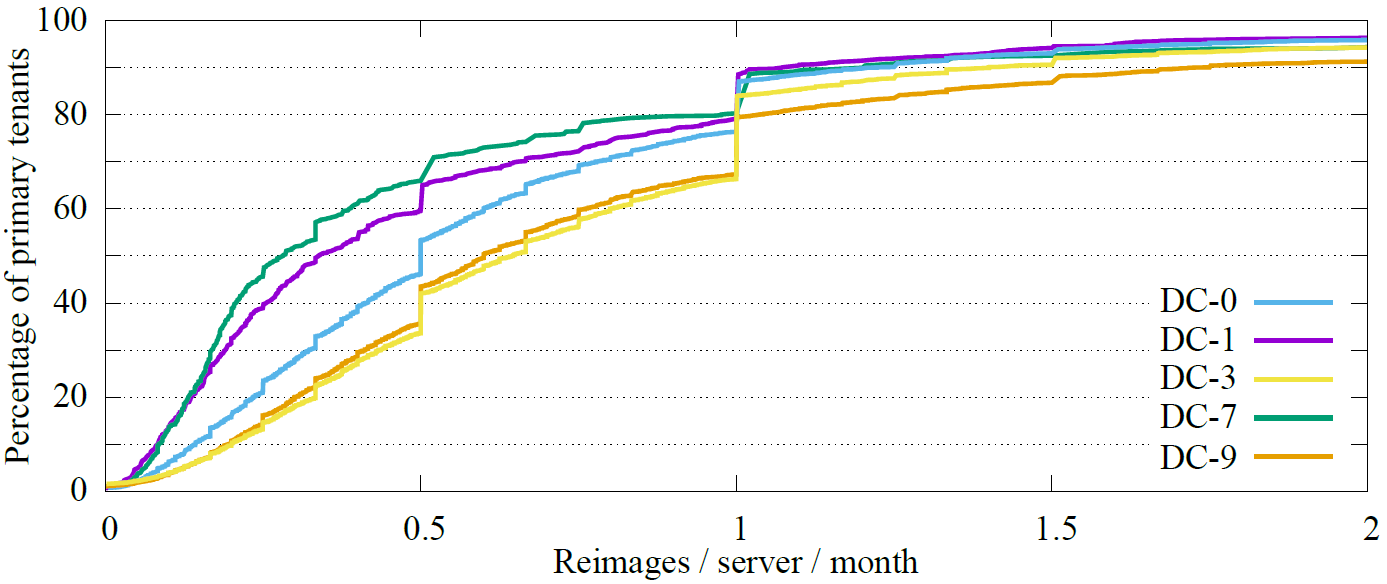
\includegraphics[width=0.5\textwidth]{./figure/reimages2.PNG}
		\end{figure}
		\end{itemize}
	\end{frame}

%------------------------------------------------
% Co-location Techniques
%------------------------------------------------
\section{Co-location Techniques}

% Task scheduling
\subsection{Task scheduling}
	\begin{frame}
	\frametitle{History-Based Task Scheduling}
		\begin{figure}[h!]
		\centering
		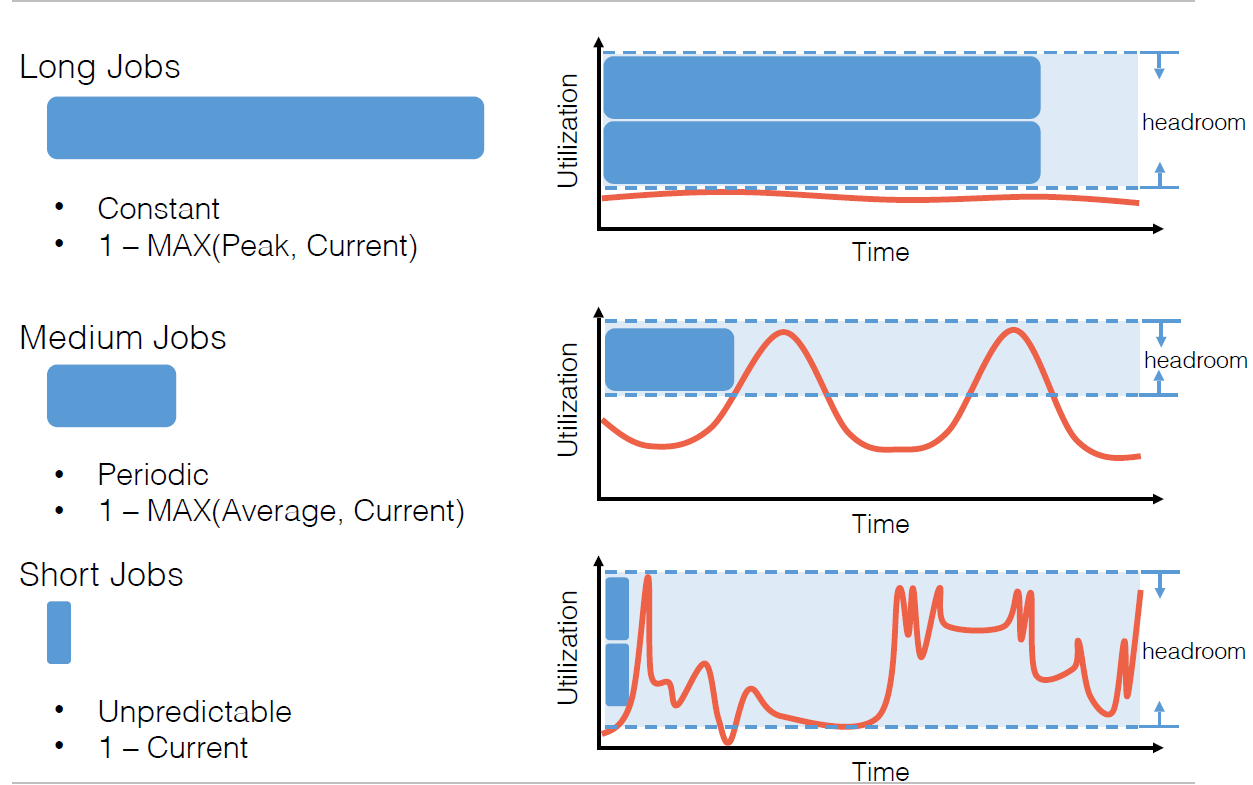
\includegraphics[width=0.9\textwidth]{./figure/task.PNG}
		\end{figure}
	\end{frame}

	\begin{frame}
	\frametitle{Task Scheduling}
		\begin{itemize}
		\item Fast Fourier Transform (FFT)
			\begin{itemize}
			\item Get 3 patterns.
			\end{itemize}
		\item Clustering algorithm
			\begin{itemize}
			\item K-means algorithm
			\item Average and peak utilizations
			\end{itemize}
		\item Class selection algorithm
		\end{itemize}
	\end{frame}

	\begin{frame}
	\frametitle{Class Selection Algorithm}
		\begin{figure}[h!]
		\centering
		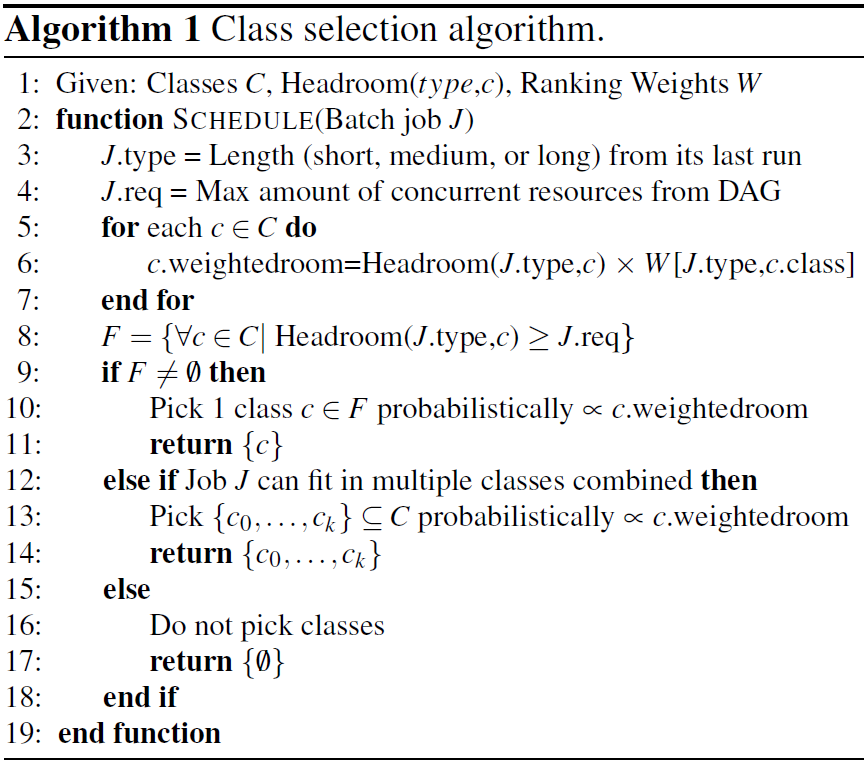
\includegraphics[width=0.6\textwidth]{./figure/algorithm1.PNG}
		\end{figure}
	\end{frame}

% Data placement
\subsection{Data placement}
	\begin{frame}
	\frametitle{History-Based Data Placement}
		\begin{itemize}
		\item Data availability
			\begin{itemize}
			\item Diverse in utilization pattern.
			\end{itemize}
		\item Data durability
			\begin{itemize}
			\item Diverse in reimaging pattern.
			\end{itemize}
		\end{itemize}
		\begin{figure}[h!]
		\centering
		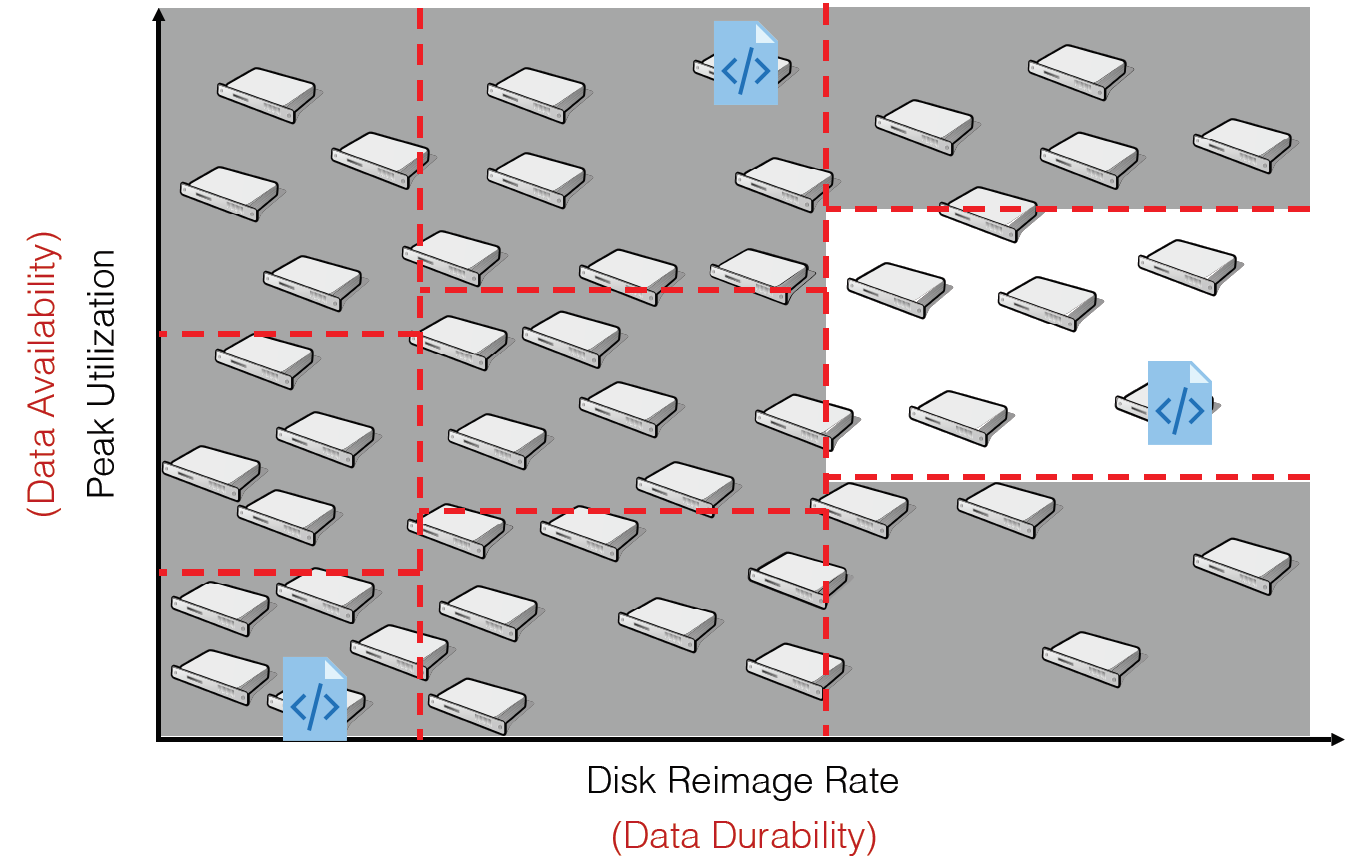
\includegraphics[width=0.5\textwidth]{./figure/data.PNG}
		\end{figure}
	\end{frame}

	\begin{frame}
	\frametitle{Replica Placement Algorithm}
		\begin{figure}[h!]
		\centering
		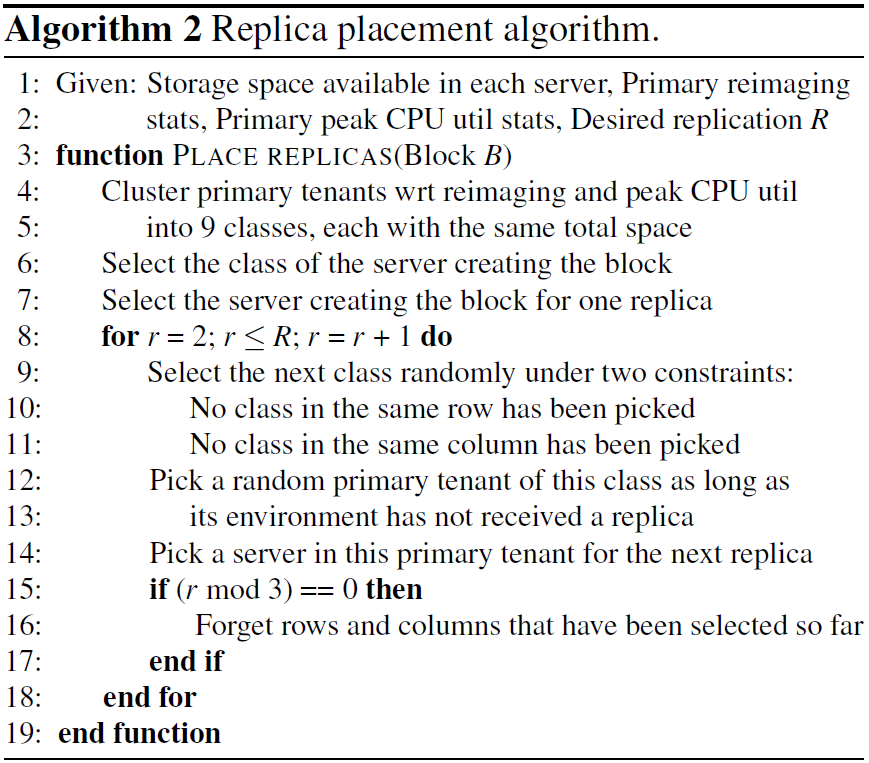
\includegraphics[width=0.6\textwidth]{./figure/algorithm2.PNG}
		\end{figure}
	\end{frame}

%------------------------------------------------
% Experiment
%------------------------------------------------
\section{Experiment}

% Implementation
\subsection{Implementation}
	\begin{frame}
	\frametitle{System Implementation}
		\begin{itemize}
		\item Overview of YARN-H, Tez-H, and HDFS-H in a co-location scenario.
		\end{itemize}
		\begin{figure}[h!]
		\centering
		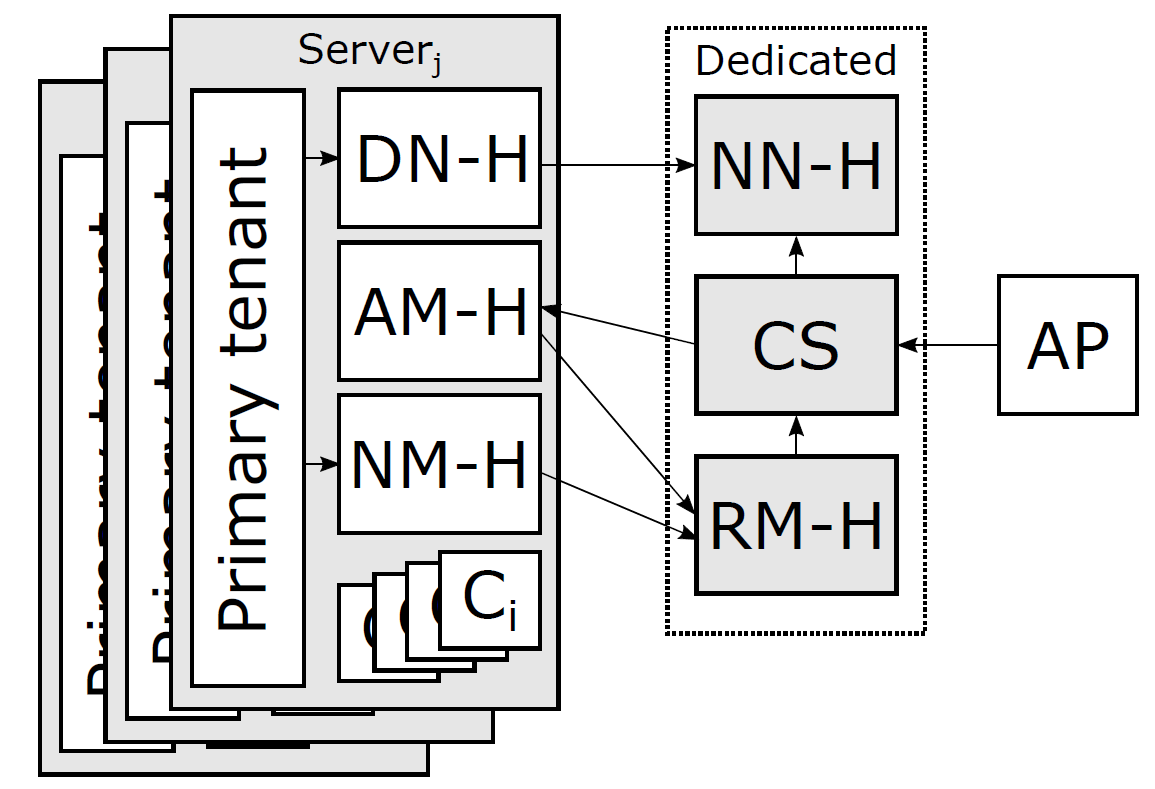
\includegraphics[width=0.5\textwidth]{./figure/implements.PNG}
		\end{figure}
	\end{frame}

% Evaluation
\subsection{Evaluation}
	\begin{frame}
	\frametitle{Evaluation}
		\begin{itemize}
		\item Environment:
			\begin{itemize}
			\item 102-server cluster
			\end{itemize}
		\item Primary tenant (interactive service):
			\begin{itemize}
			\item Apache Lucene search engine with utilization trace
			\end{itemize}
		\item Batch task:
			\begin{itemize}
			\item TPC-DS benchmark
			\end{itemize}
		\end{itemize}
	\end{frame}


% Experiment
\subsection{Experiment}
	\begin{frame}
	\frametitle{Batch Task Scheduling}
		\begin{itemize}
		\item Interactive services performance
			\begin{figure}[h!]
			\centering
			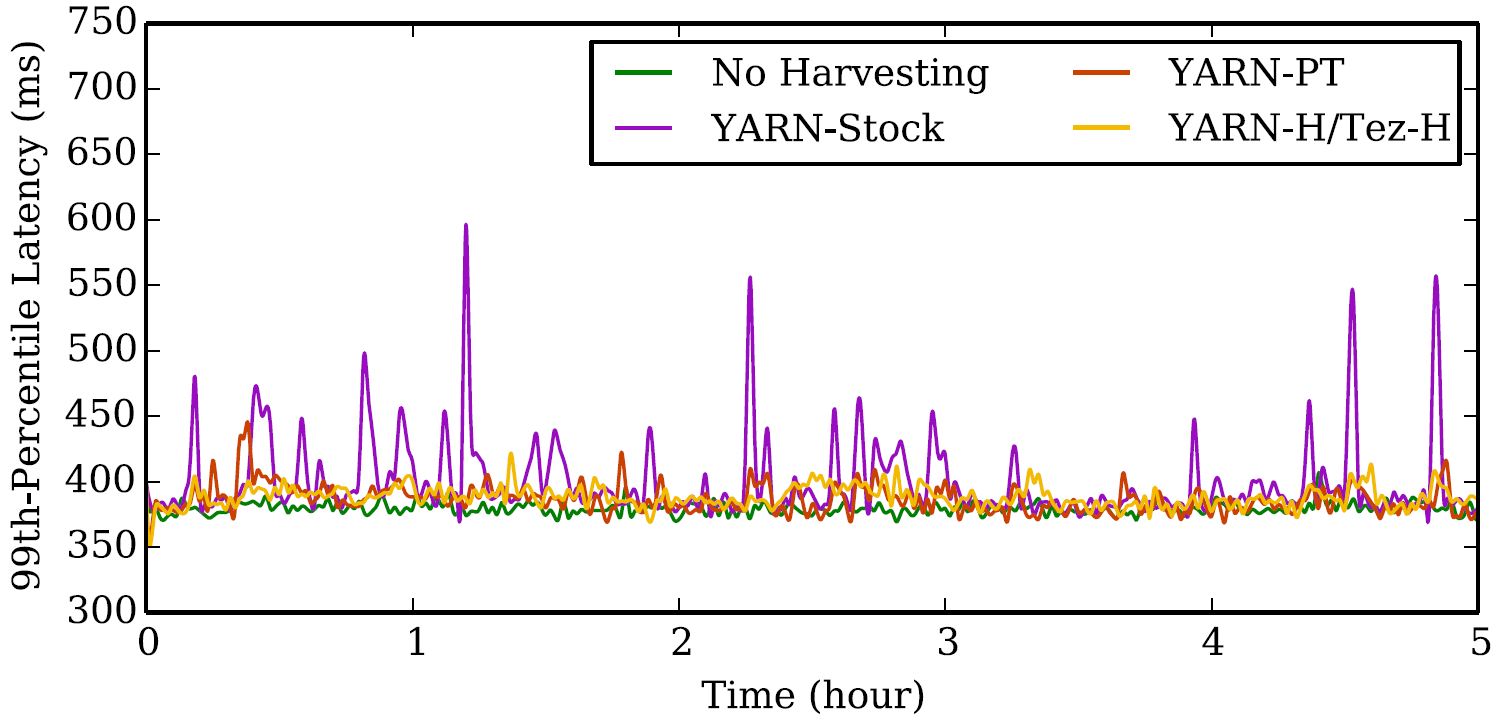
\includegraphics[width=0.5\textwidth]{./figure/experiment1.PNG}
			\end{figure}
		\item Job duration - reducing task killing
			\begin{figure}[h!]
			\centering
			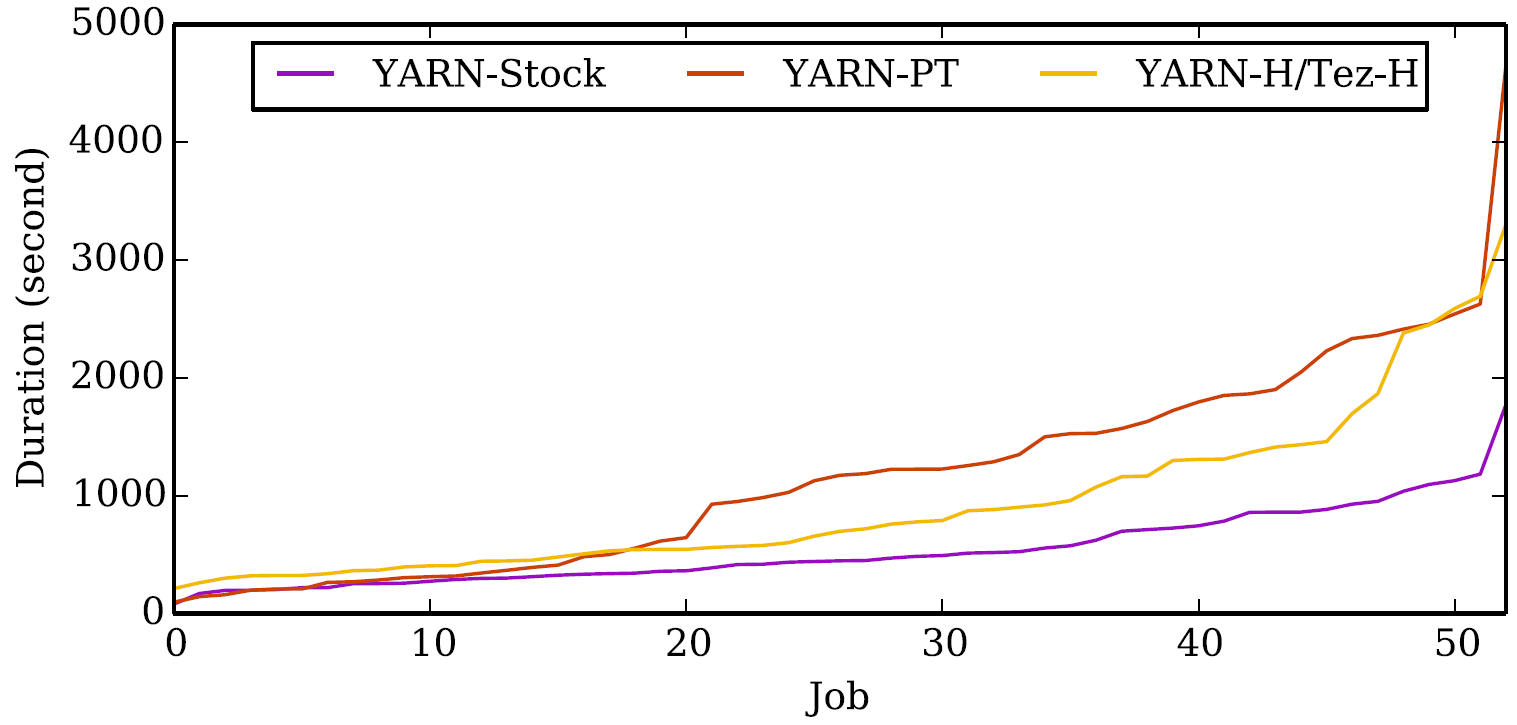
\includegraphics[width=0.5\textwidth]{./figure/experiment2.PNG}
			\end{figure}
		\end{itemize}
	\end{frame}

	\begin{frame}
	\frametitle{Data Placement}
		\begin{itemize}
		\item Data availability
			\begin{figure}[h!]
			\centering
			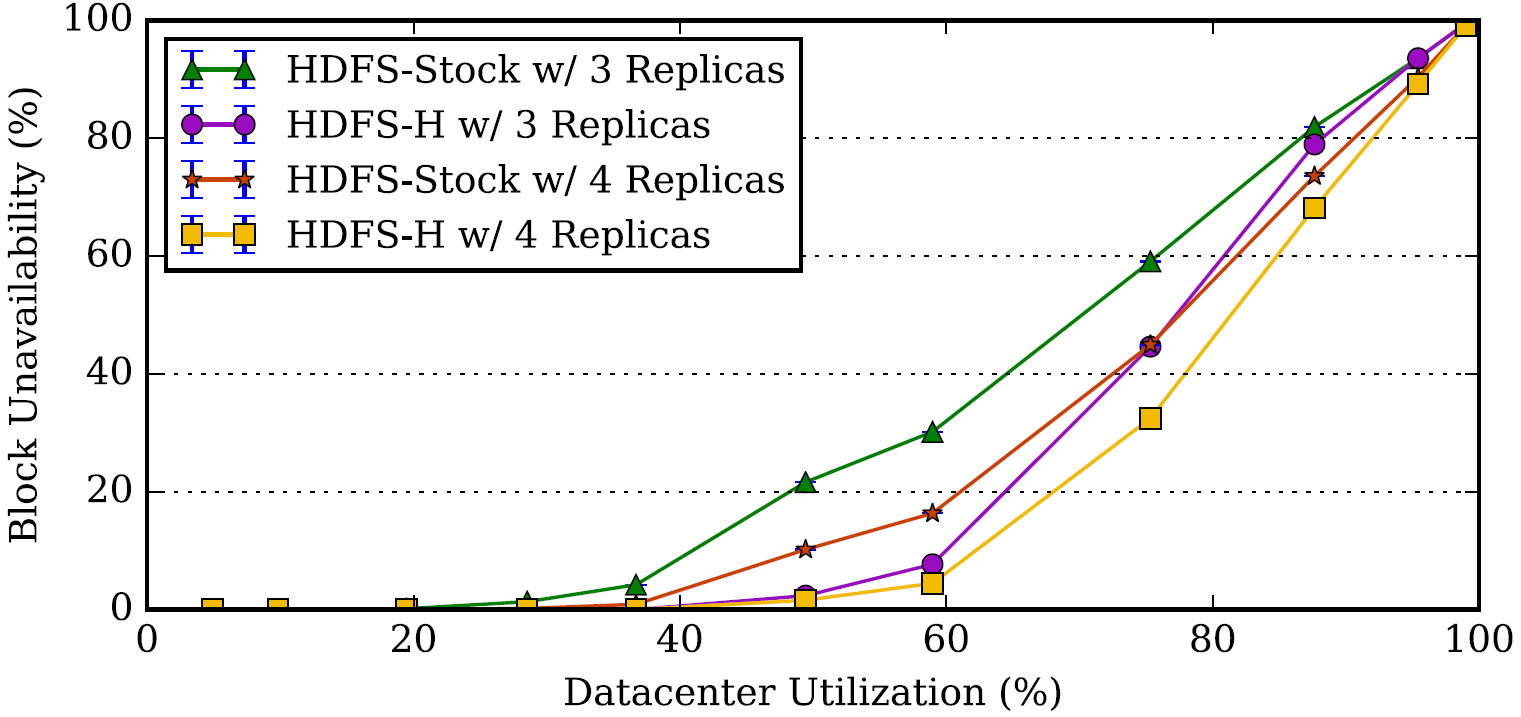
\includegraphics[width=0.5\textwidth]{./figure/experiment3.PNG}
			\end{figure}
		\item Data durability
			\begin{figure}[h!]
			\centering
			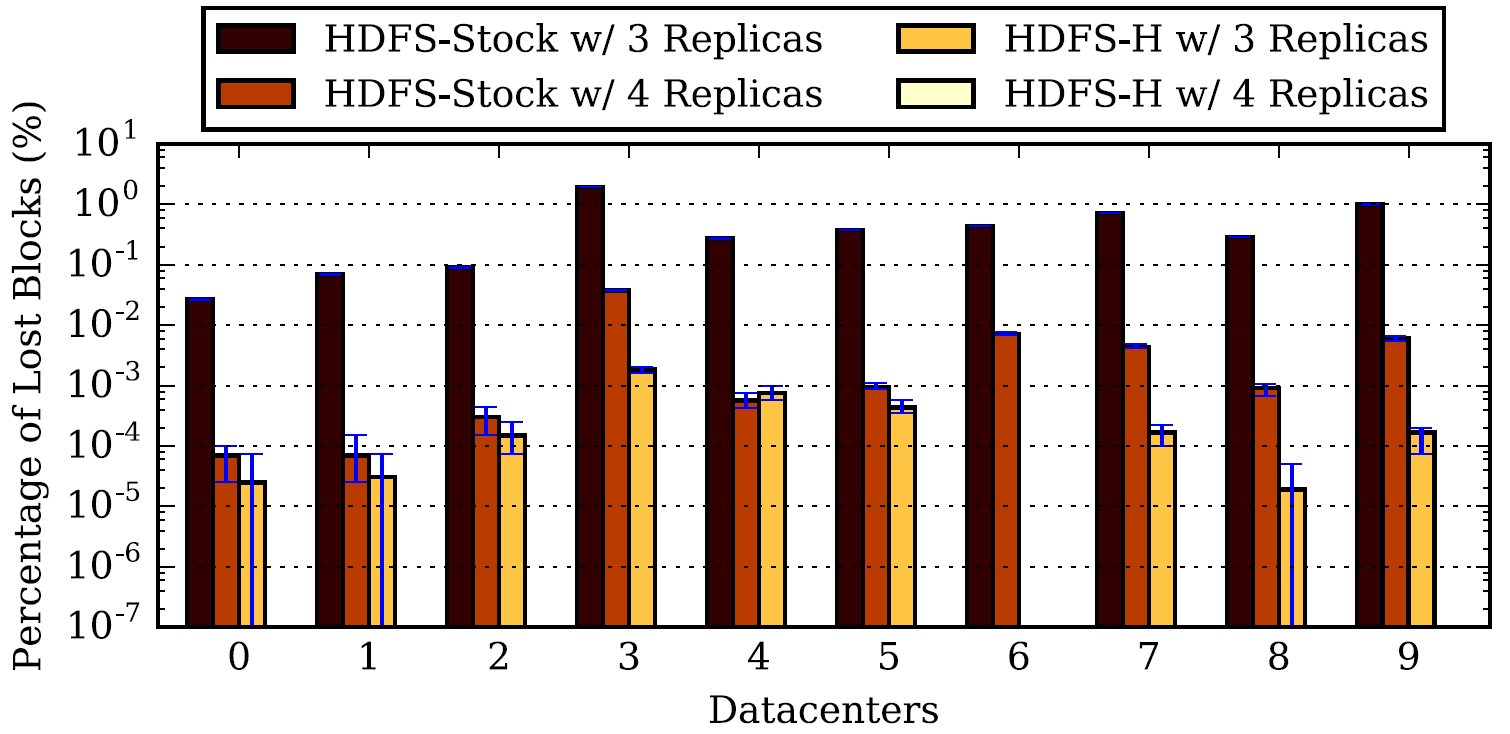
\includegraphics[width=0.5\textwidth]{./figure/experiment4.PNG}
			\end{figure}
		\end{itemize}
	\end{frame}

%------------------------------------------------
% Conclusion
%------------------------------------------------
\section{Conclusion}

\subsection{Conclusion}
	\begin{frame}
	\frametitle{Conclusion}
		\begin{itemize}
		\item Embody knowledge of the existing primary workloads, and leverage historical utilization.
		\item Improve batch job performance while protecting primary workloads.
		\item Eliminate data loss and unavailability in many scenarios.
		\end{itemize}
	\end{frame}

\subsection{Future work}
	\begin{frame}
	\frametitle{Future Work}
		\begin{itemize}
		\item Paper
			\begin{itemize}
			\item Isolation and security in public cloud.
			\end{itemize}
		\item Project
			\begin{itemize}
			\item Network utilization.
			\item Constraint of Ethernet bandwidth.
			\end{itemize}
		\end{itemize}
	\end{frame}

\end{document} 
